% $Header: https://svn.ita.chalmers.se/repos/security/edu/course/computer_security/trunk/assignment/3/template/latex/report.tex 611 2013-02-20 13:33:23Z pk@CHALMERS.SE $
%
%

\documentclass[a4paper,twoside,11pt]{article}

\usepackage{etoolbox}
\usepackage[utf8]{inputenc}
\usepackage{microtype}

\usepackage[pdftex,hidelinks]{hyperref}
\hypersetup{
    pdfstartview=FitH,
%    pdftitle={},
%    pdfauthor={},
%    pdfsubject={},
%    pdfkeywords={}
%    bookmarks,
%    bookmarksopen,
%    colorlinks,
%    linkcolor=blue,
%    citecolor=blue,
%    urlcolor=magenta,
}
\usepackage[english]{babel}
\usepackage[T1]{fontenc}
\usepackage{geometry}
\usepackage{fancyhdr}


% Setup bibliography
\usepackage{csquotes}
\usepackage[backend=biber, natbib=true, maxnames=2, minnames=1, 
maxbibnames=10, minbibnames=6, citestyle=numeric-comp, sorting=none, 
firstinits=true]{biblatex}
%\providecommand{\bibfont}{\footnotesize}
%\renewcommand{\bibfont}{\footnotesize}

% To be used for colors
\usepackage{color}
\usepackage[usenames,dvipsnames,svgnames,table]{xcolor}

% Useful Packages
\usepackage{amsmath}
\usepackage{amsthm}
\usepackage{amsfonts}

\usepackage{breakurl}
\usepackage{paralist}
\usepackage{graphicx}
\usepackage{epsfig}
\usepackage{tabularx}
\usepackage{subfigure}
\usepackage[symbol]{footmisc}


\usepackage{listings}
\lstset{language=bash
    ,basicstyle=\footnotesize\ttfamily
    ,frame=single
    ,breaklines=true
    ,columns=fullflexible
    ,keepspaces=true
    ,numbers=left, numberstyle=\tiny, stepnumber=2, numbersep=5pt}

% Nice tables
\usepackage{hhline}
\usepackage{booktabs}
\usepackage{caption}

% Loading ToDo notes
\usepackage{setspace}
\usepackage{todonotes}
\newcommand{\inlinetodo}[2][]{\todo[caption={#2},inline,#1]{#2}}
\newcommand{\checknote}[2][]{\todo[caption={#2},size=\small,color=yellow!40,#1]{\begin{spacing}{0.5}#2\end{spacing}}}


\makeatletter
\renewcommand{\title}[1]{\gdef\@title{#1}}
\renewcommand{\author}[1]{\gdef\@author{#1}}
\renewcommand{\date}[1]{\gdef\@date{#1}}
\newcommand{\report}[1]{\gdef\@report{#1}}
\newcommand{\group}[1]{\gdef\@group{#1}}
\newcommand{\version}[1]{\gdef\@version{#1}}

\newcommand{\maketitlepage}{%
 \thispagestyle{empty}
 {
  \vspace{2cm}
  {\huge\centering\@title\par}
  \vspace{2cm}
  {\centering\@report\par}
  \vspace{2cm}
  {\centering\@author\par}
  \vskip1em
  {\centering\small Group~\@group\par}
  \vfill
  {\centering Version no:~\@version
   \vskip1em
   \@date\par}
  \vspace{2cm}

  \newpage
  \thispagestyle{empty}
  \mbox{}
 }
}
\makeatother

\renewcommand{\maketitle}{%
 \pagestyle{plain}
 \setcounter{page}{-100}
 \maketitlepage
 \newpage
 \pagenumbering{roman}
 \tableofcontents
 \cleardoublepage
 \pagenumbering{arabic}
}

% Title and Authors. This should be updated by you!
\title{The Linux Firewall}
\report{Laboratory Report in EDA491/DIT071 Computer Security}
\author{Simon Fransson\\Henrik Hugo}
\group{12}
\date{\today}
\version{0.1}

% The bilbiography to include
\addbibresource{mybib.bib}


\begin{document}

\maketitle % Make titlepage

\section{Introduction} 
\label{sec:intro}
Today people take Internet and being connected for granted. It is such a common part of our everyday life that if Internet would stop working tomorrow many experts claim that it would result in a societal disaster. (Danny Hillis ref) Everyone can use Internet, it is very convenient and user-friendly. What people seem to forget is that the Internet is NOT secure. Without proper protection it is very easy for an attacker to gain access to a private network. A first perimeter of defense against attackers would be to implement a firewall. A firewall help protect against attackers by denying them access and blocking security holes in your system that attackers could exploit.

This report is written to formulate and describe the problems and thoughts about how to set up a firewall using iptables on a Linux Redhat system. The purpose of this report is to introduce the reader to security threats and how these threats can partially be prevented using a firewall. It also aims to present the results obtained from the laboratory work done with iptables on Chalmers Linux Redhat systems. The configurations and thoughts about this laboratory work will also be presented.

The rest of the report is organized as follows: Section 2 presents the system configuration and requirements. Section 3 presents the firewall configuration done by the writers of this report. Section 4 aims to present reasoning as to why the specific configuration is correct. Section 5 provides some discussion regarding the firewall configuration, raising questions such as 'what could be done different?'. Section 6 presents the conclusions obtained from this labs and reflections upon the subject of firewalls.

%\inlinetodo{This section shall introduce the reader to the subject. It should include the purpose of the report, 
%i.e. a formulation of the problem to which the report provides an answer. 
%\newline
%~\ \newline
%The last paragraph should explain the structure of the report, e.g., The 
%rest of the report is organized as follows: Section~\ref{sec:setup} 
%provides\ldots\nocite{*}}

%\inlinetodo{If you need information on \LaTeX, \citep{latex-wikibook} is a 
%good place to start\ldots}


\newpage
\section{System Configuration and Requirements}
\label{sec:setup}
The system that was used for the laboratory work was a Linux Redhat computer which had the netfilter framework installed. It contains the program \verb;iptables; to configure the firewall in Linux. The system was set to run three different services, the names, service types and ports can be found in Table 1. The laboratory work consisted of configuring the firewall to meet certain security requirements stated by the lab PM. These requirements were implemented to make the system more secure. The specific requirements can be found in Table 2.

\begin{table}[h]
\centering
	\begin{tabular}{| c | c | c |}
	\hline
	 Name & Service & Port \\ \hline
	 OpenSSH & SSH Server & SSH (22) \\
	 Apache & Web Server & http (8080) \\
	 Rpcbind & portmapper & sunrpc (111) \\ 
	\hline
	\end{tabular}
	\caption{The services run on the lab system}
	\label{Service table}
\end{table}

\inlinetodo{This section should include an explanation of the system configuration and the services which are running on the host. It should also include the security requirements (as stated in the lab PM).
Make appropriate use of tables. For your convenience, an example table is given below, but its content may need to be updated.}

The host has an initial firewall configuration, as shown in 
Listing~\ref{lst:fw-init}.

\lstinputlisting[caption=Initial firewall configuration,label=lst:fw-init]{firewall-init.txt}


\newpage
\section{Firewall Configuration}
\label{sec:config}
This chapter delves into the details of what the firewall configuration looked like when the lab was finished. The chapter will be divided into subchapters explaining each 'chain' such as INPUT, OUTPUT and so on.
\subsection{Chain INPUT}
This is the chain of the firewall that inspect incoming packets destined for the host. Rule number 1-3 have not been changed. From rule 4  are the new rules defined according to the firewall specification from the lab PM. The rule number 4 makes sure to accept all incoming traffic on the loopback interface. The rule can be found on line 69 in Appendix B. Rules 5-8 makes sure to drop and log all incoming traffic that comes from private/unused addresses as these may be spoofed packets. The rules can be found on lines 70-73 in Appendix B. Rule 9-10 limits the rate of incoming ICMP echo request packets to 1 packet per second. The rule is stated on line 79-80 in Appendix B. Rule 11 accepts all TCP connections that are already established or related to some other TCP connection. In other words, it makes sure that the connections which the host initiated is not dropped by the firewall. The rule can be found on line 83 in Appendix B. Rule 12-15 makes sure the firewall accepts connections for the services displayed in Table 1. Since sunrpc also accepts UDP connections there is an extra rule added for this, the rules can be found on lines 85-88 in Appendix B. Rule 16-18 makes sure to log all incoming TCP, UDP and ICMP traffic. Rules can be found on lines 90-92 in Appendix B.

\subsection{Chain OUTPUT}
This chain inspects all outgoing packets sent from the host. Rule 1 is not changed since previously. Rule 2 accepts outoing loopback traffic, statement in script is found on line 68 in Appendix B. Rule 3-6 drop and logs all traffic sent to private/unused addresses. The statement of the rules can be found on lines 74-77 in Appendix B. Rule 7 accepts all other outgoing traffic, definition in the script can be found on line 82

\subsection{Chain LOG_DROP}
This chain was created only to achieve a clean and more readable script, the number of script lines would otherwise doubled (since one line for DROP and one line for LOG would have been required). The chain simply logs and then drops the packets that enter the chain. Definition can be found on lines 53-55.

\lstinputlisting[caption=Final firewall 
configuration,label=lst:fw-config]{firewall-final.txt}

\newpage
\section{Firewall Correctness}
\label{sec:correctness}
This chapter goes into detail of the set of rule and describes why they work and how they were verified. Making sure they work as intended.

\subsection{Scan protection}
Since the order matter when configuring rules in the firewall it is important to verify their intent. Even though all chains have a default policy of drop it is necessary to explicitly drop certain packets. Packets matching the pattern of common scan methods are explicitly dropped. This is stated on lines 62-66 in Appendix B. Blocking these packets before reaching any accept-rules ensures the intent of the blockage, even if they are targeting an open port in the firewall. Verifying the effectiveness of the rules was done by performing an XMAS- and NULL-scan against the host using the NMAP tool. The scan failed to detect any of our open ports thus the scan protection is working.

\subsection{Loopback}
The next rule is allowing all traffic on the loopback interface. Allowing us to reach local services without restriction. The rules are stated in lines 68-69 in Appendix B. The loopback rules were tested using a local web server running on port 80. Reaching it locally was no issue but trying from the outside failed. Thus telling us it is working as intended.

\subsection{Ping flood}
While we want to allow the outside world to ping our host we also want to limit the amount of ping requests, because otherwise it could be used to launch a denial of service attack. This was done by only accepting one ping request per second and dropping the rest. Verification was done by sending 5 ping requests per second to the host. This resulted in a limited number of replies. We could also verify that the rules were working by seeing how many packets matched the rules in the firewall. The ping rules are stated on lines 79-80 in Appendix B.

\subsection{Stateful inspection}
It is important than the firewall allows us to initiate connections to the outside of the firewall. It is also necessary that we receive replies on connections initiated by us, making the firewall stateful. The rules allowing this are stated on lines 82-82 in Appendix B. Testing the rules was done by accessing google.com through a web browser. Thus ensuring that we can establish a TCP connection to google.com.

\subsection{Local services}
Testing SSH and web-access through port 8080 was as simple as accessing the services from the outside. Assuring us that we can reach the services. Rules for the local services are stated on lines 85-88 in Appendix B.






%\inlinetodo{Explain which tool you used and how it helped you in verifying your firewall configuration. Elaborate on why the firewall is correctly configured and does what it should do. E.g., by trying the command XXX, we found that there are only YYY number of packets returned when pinging the host. Thus, the ping protection (rule Z) is working. \\
%Also answer:\\
%-- Why is the order of your firewall rules correct and makes sense?\\
%-- Is your configuration stateful?}



\newpage
\section{Discussion} 
\label{sec:discussion}

The final firewall configuration workers as intended, blocking unwanted traffic while still allowing the user to communicate outwards. The order of the rules seems logical by explicitly blocking unwanted packets, allowing wanted and dropping the rest. Although sufficient it may not be enough for the future. New threats and type of attacks may be discovered. Maintenance may be required to ensure proper protection.

%Iptables is a very useful part of Linux, although somewhat tricky to configure. It requires concern on in what order rules are placed, what should be allowed and what should be explicitly dropped. Although powerful, it relies on the user to configure it in a correct manner.

\subsection{Further protection}
There are a few things that we could implement to improve the firewall even further. One of these is limiting the damage in the case of an intrusion by limiting outgoing traffic. Malicious programs, like botnets, tend to have patterns and use specific ports in their network communication. Known ports malicious ports are a good idea to block. Some malicious programs might start to try and participate in a distributed denial of service attack (DDoS). Limiting the amount of outgoing connection attempts might mitigate the attack before it reaches its target. Cyber attacks like DDoS are illegal in some countries and legal measures may apply to the owner of an infected computer or network.\\
\\
Although a good practice to implement it may be hard for the average user to know of such patterns and malicious ports. Measures which blocks specific communication by pattern may be better implemented on a gateway or router level. Thereby protecting all computers within a network and allowing for easier management.

\subsection{Lessons learned}
One thing we learned from this lab is that the order matters when defining your rules. Some rules may overrule others so it is also important to test your firewall configuration. Your firewall requires verification, the rules might not work as intended. New rules may affect older rules so it is important to keep a logical order in your configuration. In our configuration we started by defining what should be explicitly dropped and then what we want to allow and finally a default drop on packets not matching any rules.
\\
\\
Our final firewall configuration may not be complete but it is a good start for a safer connection to the internet. Other purposes, like running secure services on a server, will require a different firewall configuration.


%\inlinetodo{Reflect on the current firewall configuration. E.g., is it complete? What have you learned? Recommendations for future configuration, maintenance requirements of the firewall, etc.}



\newpage
\section{Conclusion} 
\label{sec:conclusion}
Setting up proper security is not an easy task. It is easy to make a statement and say that a system is secure. However a system can never be secure, the real question is HOW secure the system is. The conclusions that can be drawn from the laboratory work are that a firewall is a very good first step into making a system more secure. It is fairly easy to configure with a software such as \verb;iptables;. The firewall can help in blocking unwanted incoming connections. It helps in restricting what kind of applications that are allowed, tightening up eventual security holes. As shown in the report it can also help against attacks such as ping floods and probing of ports using XMAS or NULL scans. Considering that it takes about two hours to construct a firewall that achieves this it seems very unwise to not do it.

A firewall is one essential tool in minimizing security threats in your system. As shown in the report it helps not only denying access to unwanted users but can also log these attempts. It helps the administrator in observing the eventual security threats pointed towards the system. It is the first perimeter of defense and in the task of achieving a more secure system we believe it is the first thing to implement.
%\inlinetodo{Present your conclusions in relation to the objective stated in the introduction. It should not contain new information that is not discussed elsewhere in the report. }



\newpage

\printbibliography
\addcontentsline{toc}{section}{References}

%\inlinetodo{Please use Vancouver/IEEE style for your referencing. For more
%information please check: 
%\burl{http://www.lib.unimelb.edu.au/cite/ieee/index.html}. References can 
%easily be managed with the program \texttt{JabRef}.}
\appendix
\newpage
\section{Initial Firewall Configuration} \label{app:fw-init}

The initial configuration script of the firewall is shown in
Listing~\ref{lst:fw-init-script}.

\lstinputlisting[caption=Initial firewall 
configuration script,label=lst:fw-init-script]{firewall-init.sh}

\newpage
\section{Final Configuration Script} 
\label{app:fw-final}

The final configuration script of the firewall is shown in
Listing~\ref{lst:fw-final-script}.

\lstinputlisting[caption=Final firewall configuration script,label=lst:fw-final-script]{firewall-final.sh}

\newpage
\section{Answers to Assignment Questions}

\noindent \textbf{Q1. After DROPping echo-reply packets on OUTPUT chain, what 
was the observed effect? Use Figure~\ref{fig:icmpexampleQ1} to illustrate the 
path of the packets. Mark the path with arrows and use an X to mark the point 
where the packets are DROPped.}
~\ \\

The host is receiving incoming echo requests and replies with and echo reply. However, outgoing echo replies are dropped when matching the newly created rule (as marked by the red X in figure \ref{fig:icmpexampleQ1} ).
~\ \\

\noindent \textbf{Q2. After DROPing echo-request packets on INPUT chain, what
was the observed effect? How is this reaction different from the reaction
achieved in Q1? Use Figure~\ref{fig:icmpexample} to illustrate the path of 
the
packets. Mark the path with arrows and use an X to mark the point where the
packets are DROPped.}
~\ \\

This time around incoming echo requests will be blocked going in to our host.
~\ \\

\begin{figure}[!ht]
    \begin{center}
        \subfigure[Use this Figure to explain Q1]{
            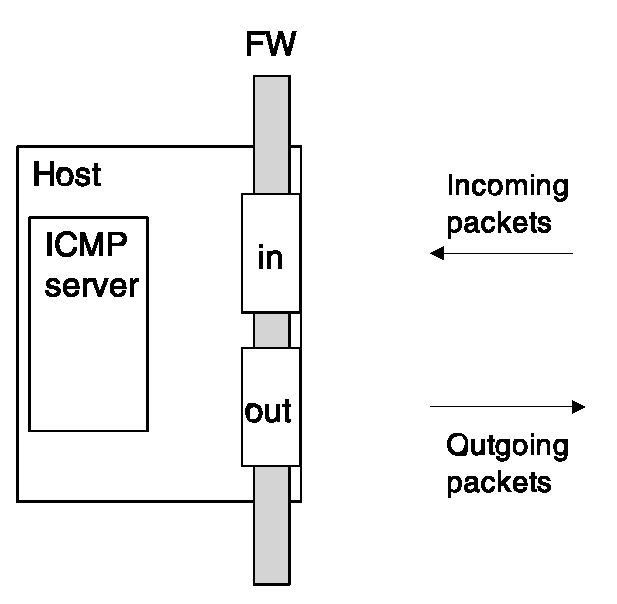
\includegraphics[scale=0.5]{figures/icmpexample.eps}
            \label{fig:icmpexampleQ1}
        }
        \hspace{1in}
        \subfigure[Use this Figure to explain Q2]{
            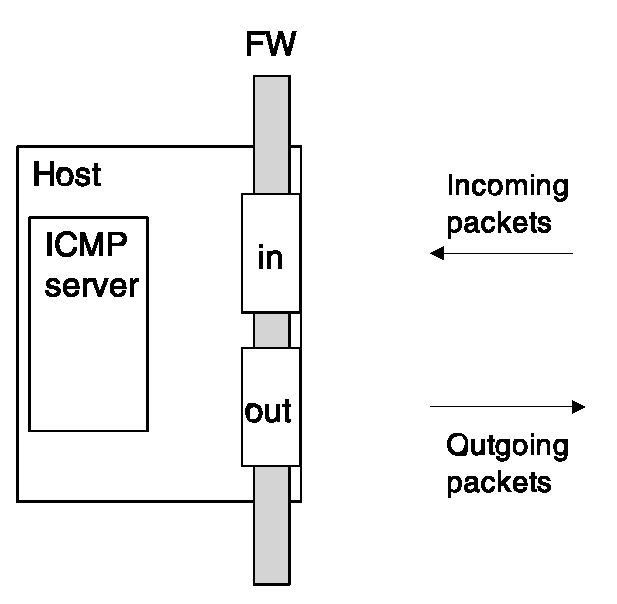
\includegraphics[scale=0.5]{figures/icmpexample.eps}
            \label{fig:icmpexampleQ2}
        }
    \end{center}
    \caption{Figure to help you illustrate your thoughts regarding the packet 
        flow in questions Q1 and Q2.}
    \label{fig:icmpexample}
\end{figure}

\noindent \textbf{Q3. For each entry in the log, several information items are
displayed. Some entries can be useful for creating new rules. Explain the 
items \texttt{IN}, \texttt{OUT}, \texttt{SRC}, \texttt{DST} and \texttt{PROTO}
mean and why these might be useful.}
~\ \\

IN and OUT denotes on what physical interface the packet entered and/or exited. SRC and DST represents the source and destination ip addresses respectively. PROTO is the protocol used on the network layer. This can be either TCP or UDP. (Table??)
~\ \\

\noindent \textbf{Q4. At this stage, with default policy set to DROP for all 
chains, would you consider the system secure? Would you consider it useful?}
~\ \\

The system is indeed more secure with the default policy set to DROP, not allowing any traffic going either in or out. In the aspect of being useful, a local user would not be permitted to browse the web or even check their mail at this stage.
~\ \\

\noindent \textbf{Q5. Assume instead that you used default policy ACCEPT, 
would you consider the system secure now? Would you consider it useful?}
~\ \\

With a default policy set to ACCEPT the system would be less secure. Having no control over who has access or from where. Local users and processes would not have any issue connecting to the outside world making it convenient. 
~\ \\

\noindent \textbf{Q6. You just added some protection against flooding by 
limiting the number of packets the firewall will let through to 1 per second. 
Give two examples on how you can tell that you are protected!}
~\ \\


\end{document}
